\chapter{Das EVM8168-Entwicklungsboard}
\label{ch:board}
\rm

F�r die in den folgenden Kapiteln beschriebenen Arbeitsschritte zur Optimierung und Analyse des Programmes wurde ein EVM8168-Entwicklungsboard verwendet, welches von der Firma Texas Instruments in Zusammenarbeit mit der Firma Spectrum Digital entwickelt wurde.
Dieses Board kann mit Hilfe eines DM816x (DaVinci\texttrademark) ARM-Prozessors entweder selber Programme ausf�hren oder es k�nnen auch die beiden ARM-Prozessoren C6A816x (Integra\texttrademark) oder AM389x (Sitara\texttrademark) emuliert werden. 


\section{Aufbau des EVM8168} \label{sec:evm816}
Wie in \cite{spec} beschrieben bietet das EVM816x-Entwicklungsboard eine Standalone-Plattform um Programme f�r DaVinci\texttrademark, Integra\texttrademark~oder Sitara\texttrademark~Prozessoren der Firma Texas Instruments zu entwickeln und zu debuggen. Hierf�r sind neben dem DaVinci\texttrademark~noch weitere On-Board Peripherie auf dem Board aufgebracht, die im folgenden teilweise n�her erkl�rt werden sollen.
Das EVM8168-Board hat unter anderem folgende Komponenten integriert:

\begin{itemize}
	\item DM816x- (DaVinci\texttrademark-)ARMprozessor (\textbf{Kapitel~\ref{sec:davinci}}) mit NEON-Einheit (\textbf{Kapitel~\ref{subsec:neon}}) und DSP (\textbf{Kapitel~\ref{subsec:dsp}})
	\item 1 GB DDR3-RAM
	\item AC31061-Audiochip
	\item Gigabit Ethernet
	\item HDMI
	\item VGA
	\item USB

\end{itemize}

\textbf{Abbildung~\ref{fig:top_ti816x_evm}} zeigt eine Draufsicht auf das Entwicklungsboard und die unterhalb dessen angebrachte Daughtercard mit weiteren Anschlussm�glichkeiten.

\begin{figure}[htbp]
	\centering
		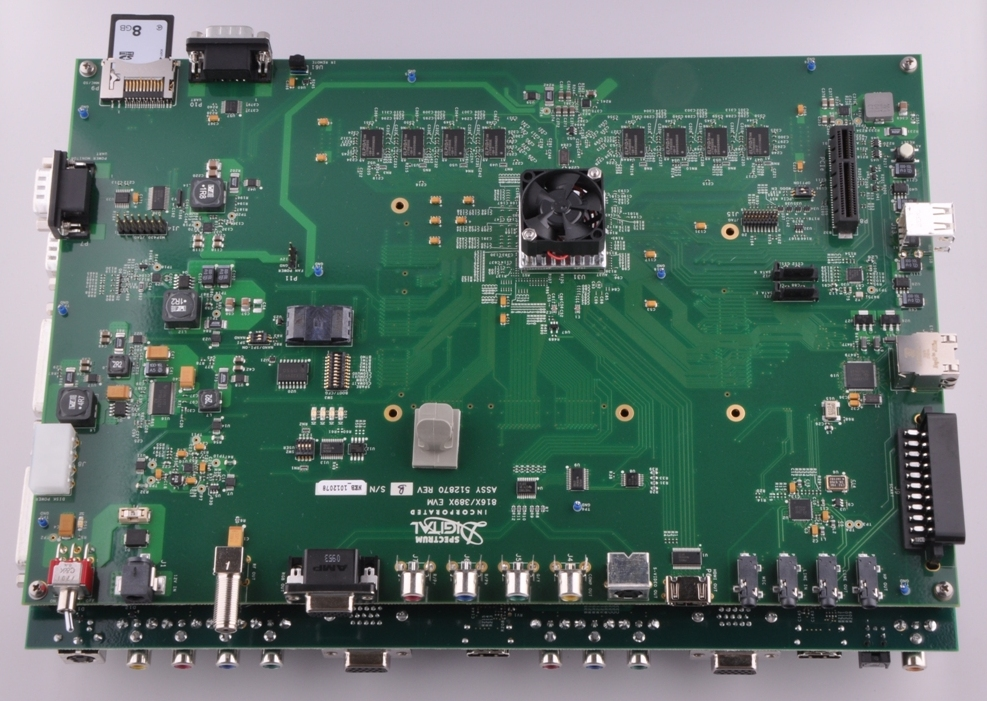
\includegraphics[scale=0.4]{../Pictures/top_ti816x_evm.png}
	\caption{Draufsicht auf das EVM8168}
	\label{fig:top_ti816x_evm}
\end{figure}



\section{Der DaVinci\texttrademark}\label{sec:davinci}
Bei dem auf dem EVM816x verwendeten ARM-Prozessor DM816x handelt es sich um einen eigentlich f�r die Videoprozessierung optimierten Prozessor der DaVinci\texttrademark-Familie von Texas Instruments.\\
Der DM816x ist ein Dualcore-Prozessor, der aus einer heterogenen Architektur basiert. \\
Zum einen enth�lt dieser einen ARM Cortex\texttrademark-A8 Risc Prozessor mit bis zu 1,35 GHz Taktung, welcher auf der ARMv7 Architektur basiert, was bedeutet, dass es sich um einen superscalaren Prozessorkern handelt und er der NEON\texttrademark Multimedia Architektur entspricht. Dieser besitzt 32K-Byte Instruction- und Datacaches, sowie einen 256K-Byte gro�en L2 Cache. Des weiteren sind noch 64K-RAM und 48K-Byte Boot ROM vorhanden (n�heres in \textbf{\ref{subsec:a8}}).\\
Als zweiter Prozessorkern enth�lt der DM816x einen C674x VLIW DSP mit bis zu 1,125 GHz Taktung. Das besondere An diesem DSP ist, dass der vollst�ndig softwarekompatibel mit DSPs der C67x+\texttrademark und C64x+\texttrademark Reihen von Texas Instruments ist (n�heres in \textbf{\ref{subsec:dsp}})\cite{evm8168}.

\subsection{ARM Cortex-A8}\label{subsec:a8}
\subsection{Die NEON-Einheit}\label{subsec:neon}
\subsection{Der C674x-DSP-Prozessor}\label{subsec:dsp}

Der C674x ist ein Floating-Point VLIW DSP mit 64 General-Purpose Registern mit je 32-Bit. Er besitzt sechs ALU Funktionseinheiten mit 32 und 40 Bit. Er unterst�tzt 32-Bit Floating Point Integer mit IEEE Single Precision (SP 32-Bit) und IEEE Double Precision (DP 64-Bit). Auf diesen schafft er bis zu vier SP Adds pro Takt und vier DP Adds alle zwei Takte, des weiteren kann er bis zu zwei Floating-Point approximierte reziproke oder quadratische Wurzeln pro Takt in SP oder DP berechnen.\\
Au�erdem besitzt er zwei Multiplizierer, entweder gemischt pr�zise Floating-Point oder Fixed-Point Integer berechnen k�nnen. Im Floating-Point-Modus schaffen diese folgende Berechnungen in den angegebenen Takten:

\begin{itemize}
	\item $2~SP \times SP~\rightarrow~ SP~pro~Takt$
	\item $2~SP \times SP~\rightarrow~ DP~pro~zwei~Takte$
	\item $2~SP \times DP~\rightarrow~ DP~pro~drei~Takte$
	\item $2~DP \times DP~\rightarrow~ DP~pro~vier~Takte$
\end{itemize}

Im Fixed-Point-Modus sind zwei 32x32, vier 16x16 oder acht 8x8 Multiplizierungen pro Takt m�glich.\\
Die Speicherarchitektur des C674x besteht aus zwei Ebenen, auf der Ersten sind 32K-Byte L1P und L1D RAM und Cache, auf der Zweiten 256K-Byte L2 RAM und Caches.\\
In der hier vorliegenden Architektur fungiert der DSP als Slave-Prozessor\cite{evm8168}.\linebreak
%
\begin{figure}[htbp]
	\centering
		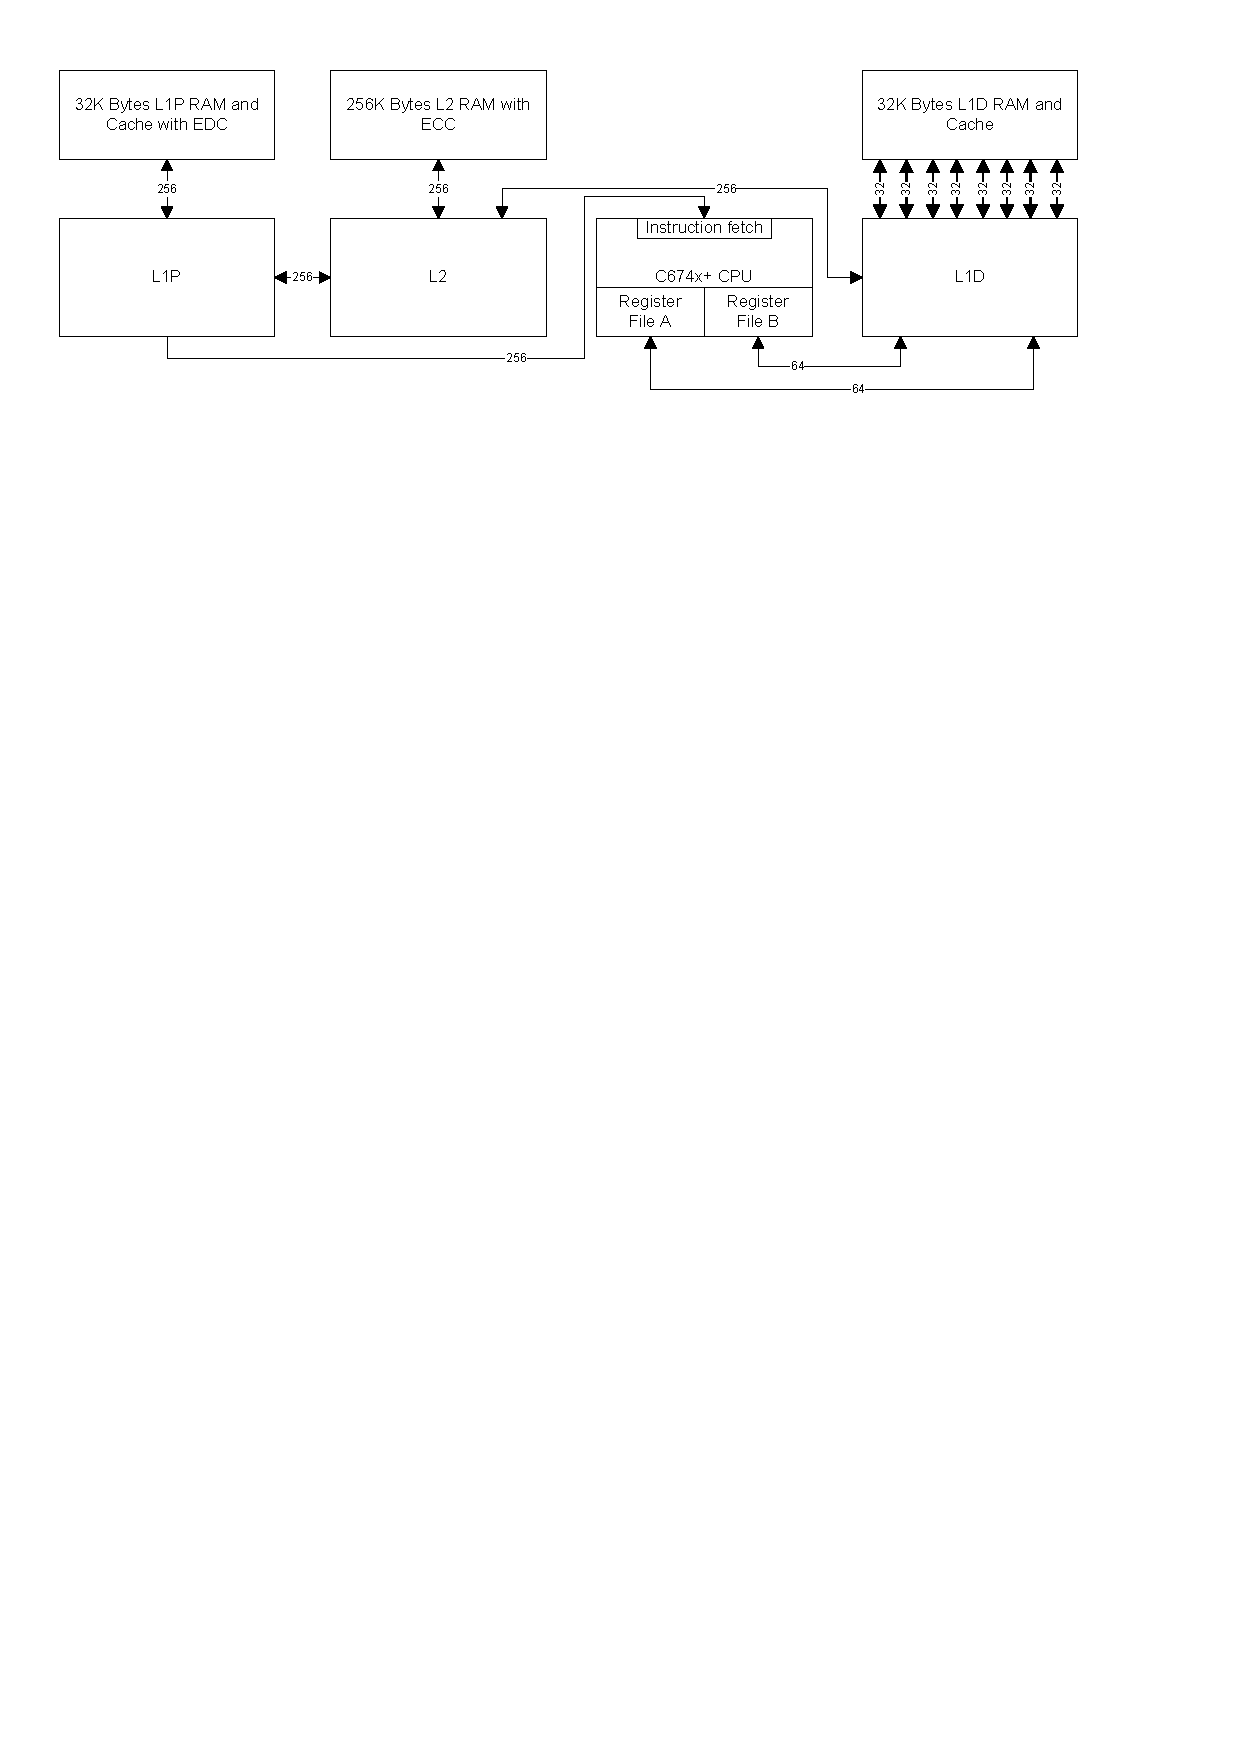
\includegraphics[width=0.65\textwidth]{../Pictures/DSPBlock.pdf}
	\caption{Blockdiagramm des C764x\cite{evm8168}}
	\label{fig:bddsp}
\end{figure}
%
Wie man dem Blockdiagramm in \textbf{Abbildung \ref{fig:bddsp}} entnehmen kann, besitzt der C674x zwei Register, die parallel Operationen ausf�hren k�nnen. Jedes dieser Register besteht hierbei aus vier Funktionseinheiten, die mit .M, .L, .D und .S bezeichnet sind. Diese Funktionseinheiten haben die Eigenschaft, dass jede von ihnen eine Operation pro Takt ausf�hren kann, diese also auch parallel ausgef�hrt werden k�nnen. Den einzelnen Einheiten sind hierbei bestimmte Operationen zugeordnet. Die einzelnen Funktionseinheiten beinhalten folgende Operationen:

\begin{itemize}
	\item .D behandelt Lade- und Speicheroperationen
	\item .S behandelt Shift-, Sprung- und Vergleichsoperationen
	\item .M behandelt Multiplikationsoperationen
	\item .L behandelt logische und arithmetische Operationen 
\end{itemize}

Somit kommen wir auf 8 Funktionseinheiten, die parallel pro Takt eine Operation durch f�hren k�nnen. Je nachdem zu welchem Register sie zugeordnet sind werden sie entweder mit einer 1 oder mit einer 2 bezeichnet, nimmt man also zum Beispiel die D Funktionseinheit des Registers A, wird diese mit .D1 bezeichnet. In \textbf{Abbildung \ref{fig:reg}} ist dieses nochmals verdeutlicht.
%
\begin{figure}[h]
	\centering
		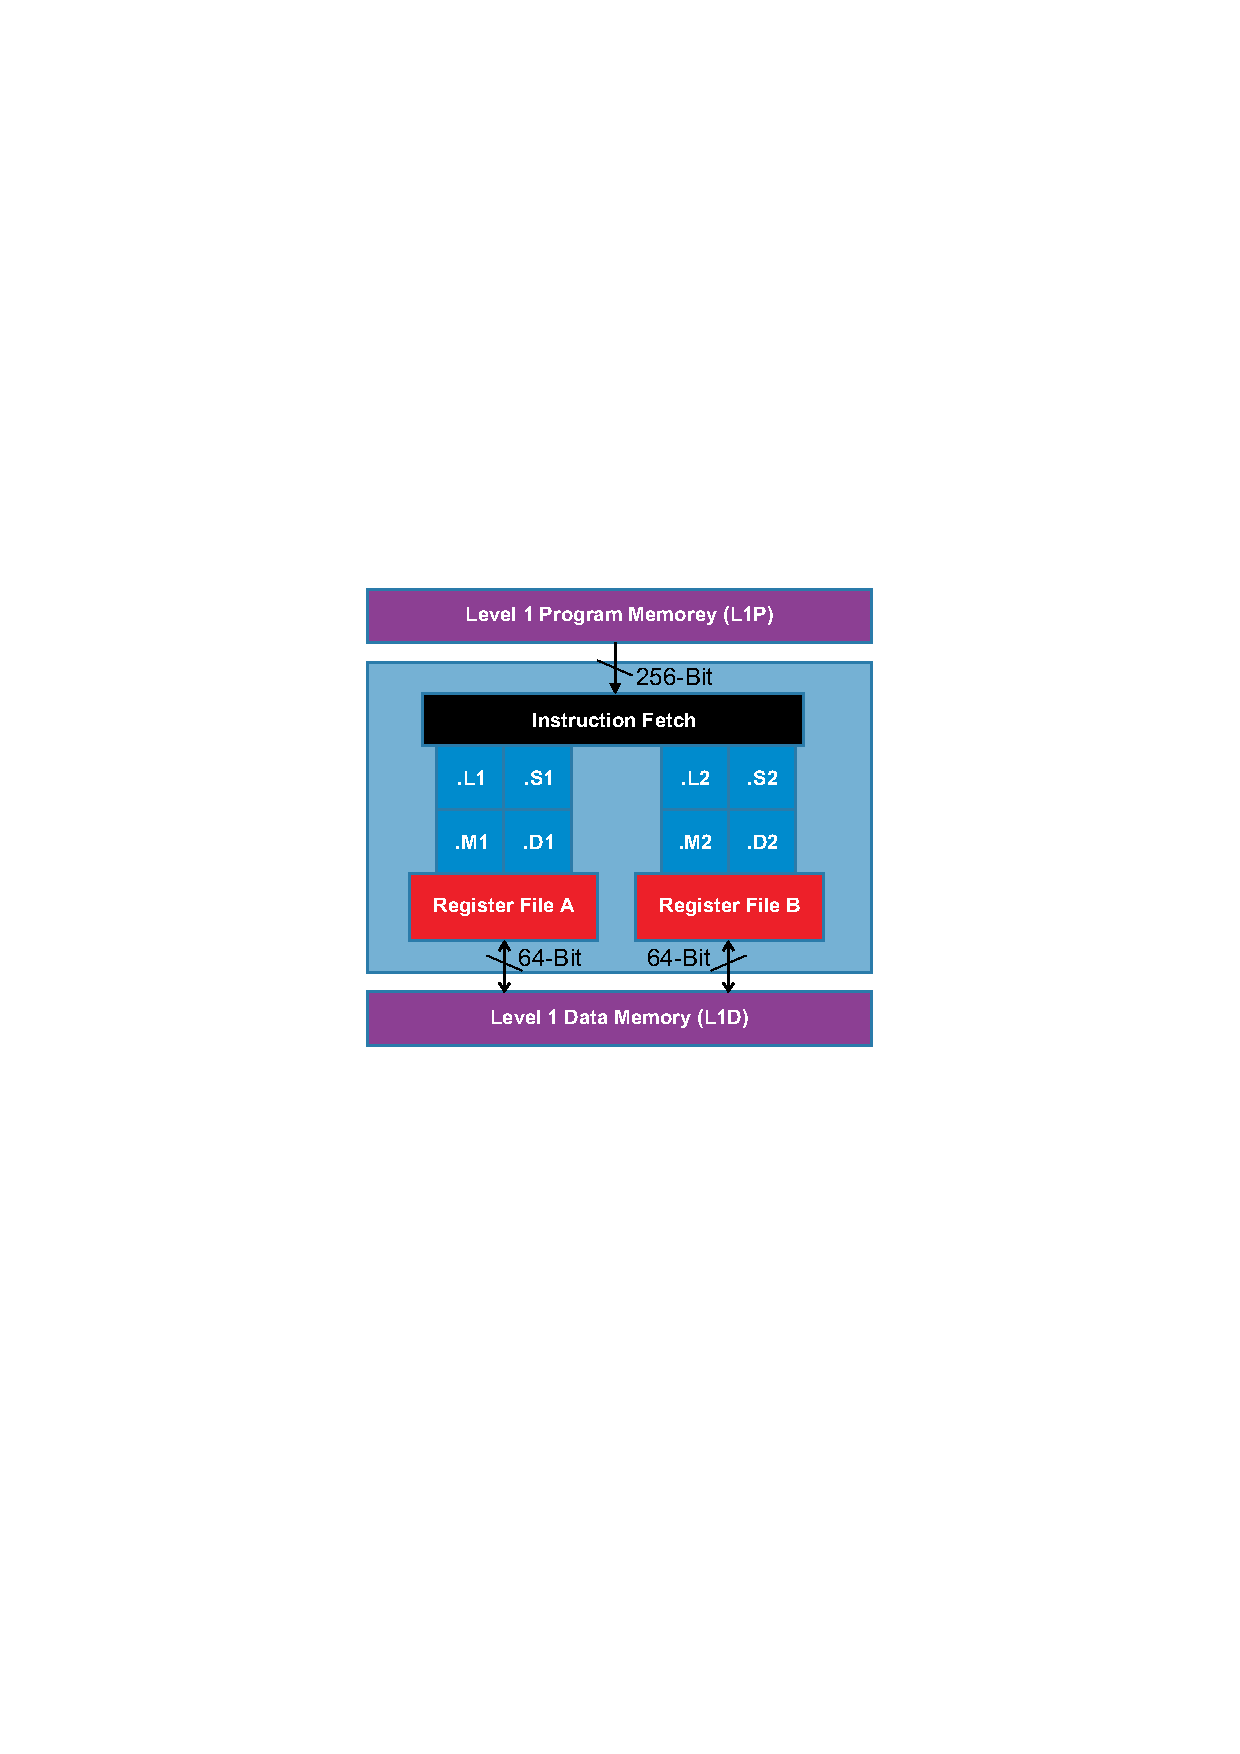
\includegraphics[scale=0.80]{../Pictures/Register.pdf}
	\caption{Registerarchitektur des C764x\cite{sprabf2}}
	\label{fig:reg}
\end{figure} 